\section{Auswertung}
Abbildung \ref{fig:spektrum} zeigt das Absortpionsspektrumpektrum des ${}^{137}\text{Cs}$-Strahlers.
Zur Erstellung der Abbildungen wird das \texttt{python}-Paket \texttt{matplotlib} \cite{Hunter:2007} verwendet, die Auswertung erfolgt
mit dem Paket \texttt{numpy} \cite{harris2020array}. Die Fehlerrechnung zur Berücksichtigung der Messunsicherheiten wird mit dem Paket \texttt{uncertainties} \cite{uncertainties}
automatisiert.
Über 
\begin{equation*}
    N = \frac{C}{t}
\end{equation*}
wird über die Anzahl der Counts $C$ auf die Zählrate $N$ umgerechnet, die als Maß für die Intensität
verwendet werden kann.
Deutlich erkennbar ist der Photopeak bei Kanalnummer 128, entsprechend der Energie $E= 662 \text{ keV}$ 
und die Compton-Kante im Bereich der Kanalnummern 85 bis 105. 
\begin{figure}
    \centering
    \includegraphics[width = \linewidth]{Leermessung.pdf}
    \caption{Spektrum der ${}^{137}\text{Cs}$-Quelle. Aufgetragen sind die Zählraten der einzelnen
    Kanäle mit den entsprechenden Kanalnummern. Die grüne Linie markiert den Photopeak bei  
    Kanalnummer 128 und der charakteristischen Energie $E_\gamma = 662 \text{ keV}$. Die Compton-
    Kante liegt im Bereich der Kanalnummern 85 bis 105. Erstellt mit dem \texttt{python}-Paket \texttt{matplotlib} \cite{Hunter:2007}.}
    \label{fig:spektrum}
\end{figure}
%TO-DO:Matrix vorher einfügen, Projektionen erklären
Die Absorptionskoeffizienten werden für die Würfel mit den Nummern 1, 3 und 4 bestimmt. Würfel 1 ist leer und besteht nur aus dem Aluminiumgehäuse.
Würfel 3 besteht nur aus einem unbekannten Material, Würfel 4 aus zwei unbekannten Materialien. 
Die gemessenen Counts $C$, Messdauer $t$, Zählraten $N$ sowie die entsprechenden Projektionen der Würfel 3 und 4 
befinden sich in den Tabellen \ref{tab:W3} und \ref{tab:W4}. Die Zählraten $N$ werden mit dem statistischen Fehler $\sqrt{N}$
belegt, die Messdauer wird als fehlerfrei angenommen.
Bei der Untersuchung von Würfel 1 werden bei einer Messdauer von $241.62 \text{ s}$ 
\begin{equation*}
    C = 37660
\end{equation*}
Counts gemessen.  
Die Berechnung der Absorptionskoeffizienten $\mu_i$ erfolgt über Gleichung \ref{eq:mu}. Über die Kovarianzmatrix $V$ ergeben sich die entsprechenden 
Unsicherheiten $\sigma_I$ als Wurzeln der Diagonalelemente
\begin{equation*}
    \sigma_{\mu_i} = \sqrt{V[\vec{\mu}_{ii}]} 
\end{equation*}
\FloatBarrier
\begin{table}[h]
    \centering
    \caption{Würfel 3, Schweres Material NOCH ÄNDERN}
    %\sisetup{table-format=1.2}
    \label{tab:W3}
    \begin{tabular}{c S[table-format=4.0] S[table-format=3.2] S[table-format=1.2]@{${}\pm{}$} S[table-format=1.2] S[table-format=1.3]@{${}\pm{}$} S[table-format=1.3]}
        \toprule
        {Projektion} & {$C$} & {$t/\si{\s}$} & \multicolumn{2}{c}{$N/\si{\s}^{-1}$} & \multicolumn{2}{c}{$\mu /\si{\cm}^{-1}$} \\
        \midrule
        $I_2$ & 1301 & 241.24 & 5.39 & 2.32 & 1.055 & 0.311\\
        $I_7$ & 1164 & 241.24 & 4.83 & 2.20 & 1.236 & 0.219\\
        $I_8$ & 594  & 241.24 & 2.46 & 1.57 & 0.858 & 0.250\\
        \bottomrule
    \end{tabular}
\end{table}
\FloatBarrier
\noindent
\FloatBarrier
\begin{table}[h]
    \centering
    \caption{Würfel 4, Unbekanntes Material NOCH ÄNDERN}
    %\sisetup{table-format=1.2}
    \label{tab:W4}
    \begin{tabular}{c S[table-format=5.0] S[table-format=3.2] S[table-format=3.2]@{${}\pm{}$} S[table-format=2.2]}
        \toprule
        {Projektion} & {$C$} & {$t/\si{\s}$} & \multicolumn{2}{c}{$N/\si{\s}^{-1}$} \\
        \midrule
        $I_1$    & 30557 & 241.80 & 126.37 & 11.24 \\
        $I_2$    & 1612  & 241.42 & 6.68   & 2.58  \\
        $I_3$    & 30303 & 241.78 & 125.33 & 11.20 \\
        $I_4$    & 10235 & 241.46 & 42.39  & 6.51  \\
        $I_5$    & 9544  & 241.46 & 39.53  & 6.29  \\
        $I_6$    & 10361 & 241.48 & 42.91  & 6.55  \\
        $I_7$    & 6993  & 241.48 & 28.96  & 5.38  \\
        $I_8$    & 6196  & 241.46 & 25.66  & 5.07  \\
        $I_9$    & 9419  & 241.56 & 38.99  & 6.24  \\
        $I_{10}$ & 7478  & 241.50 & 30.96  & 5.56  \\
        $I_{11}$ & 6377  & 241.50 & 26.41  & 5.14  \\
        $I_{12}$ & 9861  & 241.54 & 40.83  & 6.39  \\
        \bottomrule
    \end{tabular}
\end{table}
\FloatBarrier
\noindent
\FloatBarrier
\begin{table}[h]
    \centering
    \caption{Würfel 4, Unbekanntes Material Absorptionskoeffizienten NOCH ÄNDERN}
    \label{tab:W4_Abk}
    \begin{tabular}{c S[table-format=1.3]@{${}\pm{}$} S[table-format=1.3] S[table-format=1.3] S[table-format=1.3] S[table-format=1.3] S[table-format=1.3] S[table-format=1.3] S[table-format=1.3]}
        \toprule
        {} & \multicolumn{2}{c}{$\mu /\si{\cm}^{-1}$} & {$|\Delta {\mu_\text{Fe, Lit}}|$} & {$|\Delta {\mu_\text{Al, Lit}}|$} & {$|\Delta {\mu_\text{Pb, Lit}}|$} & {$|\Delta {\mu_\text{Pb, Exp}}|$} & {$|\Delta {\mu_\text{CuZn, Lit}}|$} & {$|\Delta {\mu_\text{POM, Lit}}|$} \\
        \midrule
        $\mu_1$ & 0.042  & 0.108 & 0.564 & 0.169 & 1.377 & 1.008 & 0.641 & \textbf{0.079} \\
        $\mu_2$ & 0.161  & 0.090 & 0.445 & 0.050 & 1.258 & 0.889 & 0.522 & \textbf{0.040} \\
        $\mu_3$ & 0.024  & 0.109 & 0.582 & 0.187 & 1.395 & 1.026 & 0.659 & \textbf{0.097} \\
        $\mu_4$ & 1.030  & 0.095 & 0.424 & 0.819 & 0.389 & \textbf{0.020} & 0.347 & 0.909 \\
        $\mu_5$ & 1.132  & 0.101 & 0.526 & 0.921 & 0.287 & \textbf{0.082} & 0.449 & 1.011 \\
        $\mu_6$ & 1.033  & 0.096 & 0.427 & 0.822 & 0.386 & \textbf{0.017} & 0.350 & 0.912 \\
        $\mu_7$ & 0.139  & 0.108 & 0.467 & 0.072 & 1.280 & 0.911 & 0.544 & \textbf{0.018} \\
        $\mu_8$ & -0.047 & 0.087 & 0.653 & 0.258 & 1.466 & 1.097 & 0.730 & \textbf{0.168} \\
        $\mu_9$ & 0.143  & 0.108 & 0.463 & 0.068 & 1.276 & 0.907 & 0.540 & \textbf{0.022} \\
        \bottomrule
    \end{tabular}
\end{table}
\FloatBarrier
\noindent

\begin{figure}
    \centering
    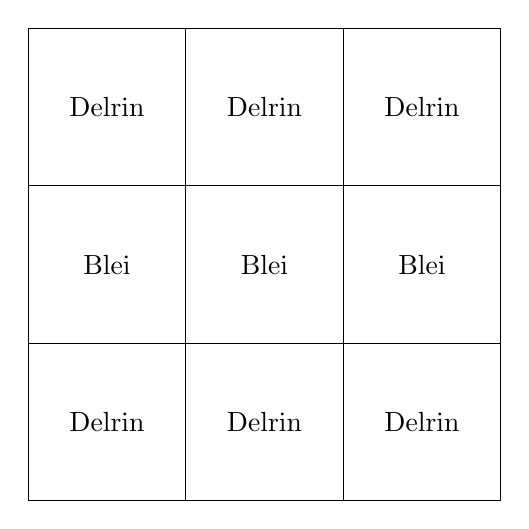
\begin{tikzpicture}
        \draw[step = 2cm,] (0,0) grid +(6,6);
        \node at (1,1) {Delrin};
        \node at (1,3) {Blei};
        \node at (1,5) {Delrin};
        \node at (3,1) {Delrin};
        \node at (3,3) {Blei};
        \node at (3,5) {Delrin};
        \node at (5,1) {Delrin};
        \node at (5,3) {Blei};
        \node at (5,5) {Delrin};
    \end{tikzpicture}
    \caption{}
    \label{fig:tikz2}
\end{figure}

\begin{figure}
    \centering
    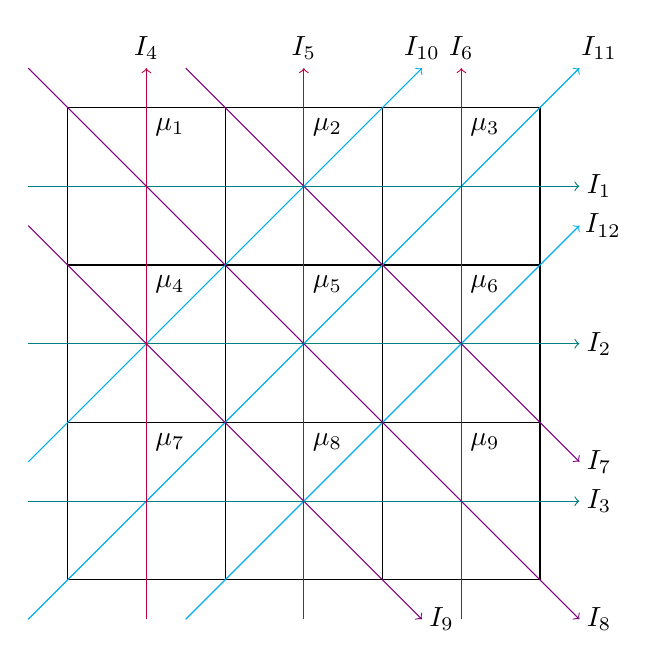
\begin{tikzpicture}
        \draw[step = 2cm] (0,0) grid +(6,6);
        \draw[->][cyan] (-0.5,-0.5)--(6.5,6.5);
        \node at (6.75,6.75) {$I_{11}$};
        \draw[->][cyan] (-0.5,1.5)--(4.5,6.5);
        \node at (4.5,6.75) {$I_{10}$};
        \draw[->][cyan] (1.5,-0.5)--(6.5,4.5);
        \node at (6.8,4.5) {$I_{12}$};
        \draw[->][violet] (1.5,6.5)--(6.5,1.5);
        \node at (6.75,1.5) {$I_{7}$};
        \draw[->][violet] (-0.5,6.5)--(6.5,-0.5);
        \node at (6.75,-0.5) {$I_{8}$};
        \draw[->][violet] (-0.5,4.5)--(4.5,-0.5);
        \node at (4.75,-0.5) {$I_{9}$};
        \draw[->][teal] (-0.5,5)--(6.5,5);
        \node at (6.75,5) {$I_{1}$};
        \draw[->][teal] (-0.5,3)--(6.5,3);
        \node at (6.75,3) {$I_{2}$};
        \draw[->][teal] (-0.5,1)--(6.5,1);
        \node at (6.75,1) {$I_{3}$};
        \draw[->][purple] (1,-0.5)--(1,6.5);
        \node at (1,6.75) {$I_{4}$};
        \draw[->][purple] (3,-0.5)--(3,6.5);
        \node at (3,6.75) {$I_{5}$};
        \draw[->][purple] (5,-0.5)--(5,6.5);
        \node at (5,6.75) {$I_{6}$};
        \node at (1.3,1.75) {$\symbf{\mu_7}$};
        \node at (1.3,3.75) {$\symbf{\mu_4}$};
        \node at (1.3,5.75) {$\symbf{\mu_1}$};
        \node at (3.3,1.75) {$\symbf{\mu_8}$};
        \node at (3.3,3.75) {$\symbf{\mu_5}$};
        \node at (3.3,5.75) {$\symbf{\mu_2}$};
        \node at (5.3,1.75) {$\symbf{\mu_9}$};
        \node at (5.3,3.75) {$\symbf{\mu_6}$};
        \node at (5.3,5.75) {$\symbf{\mu_3}$};
    \end{tikzpicture}
    \caption{}
    \label{fig:tikz1}
\end{figure}